\documentclass[../main.tex]{subfiles}

\begin{document}
\subsection{Crittografia Simmetrica: Block Cipher}
Lo schema generico della crittografia simmetrica (Symmetric block cipher) prevede che due entità (es. Bob e Alice) condividano la stessa chiave $k$. Questa chiave deve essere scambiata tramite un canale di comunicazione sicuro.

\begin{itemize}
	\item Il mittente (Bob) usa un algoritmo di cifratura $E$ per trasformare un blocco di testo in chiaro $m$ (plaintext) in un blocco cifrato $c$ (ciphertext). L'operazione è $c = E_k(m)$.
	\item Il blocco cifrato $c$ viene inviato sul canale di comunicazione insicuro.
	\item Il ricevente (Alice) usa la stessa chiave $k$ e un algoritmo di decifratura $D$ per riottenere il blocco in chiaro. L'operazione è $m = D_k(c)$.
	\item L'algoritmo di decifratura è l'inverso di quello di cifratura: $D_k = E_k^{-1}$.
	\item $m$ e $c$ sono stringhe di bit di una lunghezza fissa $b$, mentre $k$ è una stringa di bit di lunghezza $l$.
	\item Il block cipher $E_k$ definisce una relazione biunivoca (permutazione) tra i $2^b$ possibili valori di $m$ e i $2^b$ possibili valori di $c$, dipendente dalla chiave $k$.
	\item Se il messaggio è più lungo di $b$ bit, viene spezzato in una serie di blocchi $m_i$.
\end{itemize}

\begin{figure}[H]
	\centering
	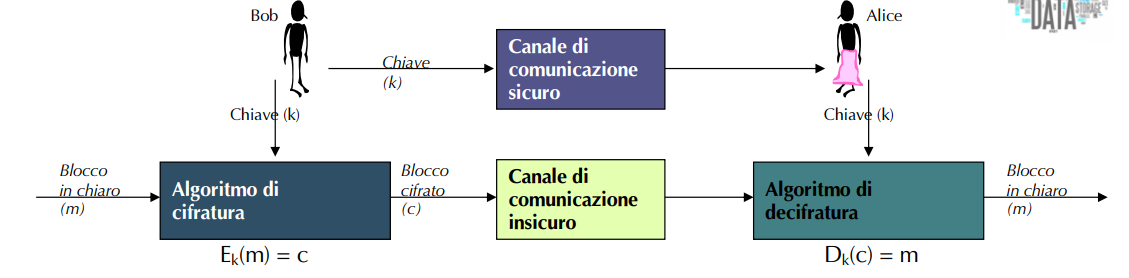
\includegraphics[width=\linewidth]{block-cypher.png}
	\caption{block cypher generico}
	\label{fig:etichetta}
\end{figure}


\subsection{Obiettivi e Tipologie dei Block Cipher}
Gli obiettivi fondamentali di un block cipher robusto sono:
\begin{itemize}
	\item \textbf{Dipendenza totale:} Ogni bit del blocco cifrato $c$ deve dipendere da tutti i bit del messaggio $m$ e da tutti i bit della chiave $k$.
	\item \textbf{Occultamento statistico:} Non ci deve essere alcuna relazione statistica evidente tra $c$ e $m$ per chi non conosce $k$.
	\item \textbf{Effetto valanga (Avalanche effect):} La modifica di un singolo bit in $m$ (o in $k$) deve portare a una modifica di ciascun bit di $c$ con probabilità 0.5.
\end{itemize}

Esistono due classi principali di block cipher:
\begin{enumerate}
	\item \textbf{Cifrario a Sostituzione:} Definisce una corrispondenza biunivoca (mappatura) tra l'insieme $M$ dei blocchi in chiaro e se stesso.
	      \begin{itemize}
	      	\item La chiave $k$ è un indice che seleziona una delle $(2^b!)$ permutazioni possibili.
	      	\item La lunghezza della chiave necessaria, $l \approx b \cdot 2^b$, rende questo approccio impraticabile (es. per $b=64$, $l \approx 2^{70}$ bit).
	      	\item Se $m_i$ si ripete, anche $c_i$ si ripete, rendendolo vulnerabile all'analisi statistica.
	      \end{itemize}
	\item \textbf{Cifrario a Trasposizione:} Effettua una permutazione (uno "shuffle") dei bit all'interno del blocco $m_i$.
	      \begin{itemize}
	      	\item Lo spazio delle chiavi è molto più ridotto: $|K| = b!$. Per $b=64$, $l \approx 384$ bit.
	      	\item Offre una segretezza ancora minore rispetto alla sostituzione, ma è un blocco costruttivo utile.
	      \end{itemize}
\end{enumerate}

\subsection{Prodotto di Cifrari: Confusione e Diffusione}
Per costruire una funzione $E_k$ complessa e sicura, si usano sostituzione e trasposizione come blocchi fondamentali in cascata (prodotto di cifrari).
\begin{itemize}
	\item Questo approccio è detto \textbf{confusione e diffusione}.
	\item \textbf{Confusione (Sostituzione):} Rende complessa la relazione tra $c$, $m$ e $k$.
	\item \textbf{Diffusione (Trasposizione):} Spalma l'informazione di un bit di $m$ su molti bit di $c$, per ottenere l'effetto valanga.
	\item Un prototipo di block cipher moderno applica ripetutamente ($t$ volte, detti \emph{round}) uno strato di sostituzione (es. $n$ S-box parallele) e uno strato di trasposizione (P-box).
\end{itemize}

\begin{figure}[H]
	\centering
	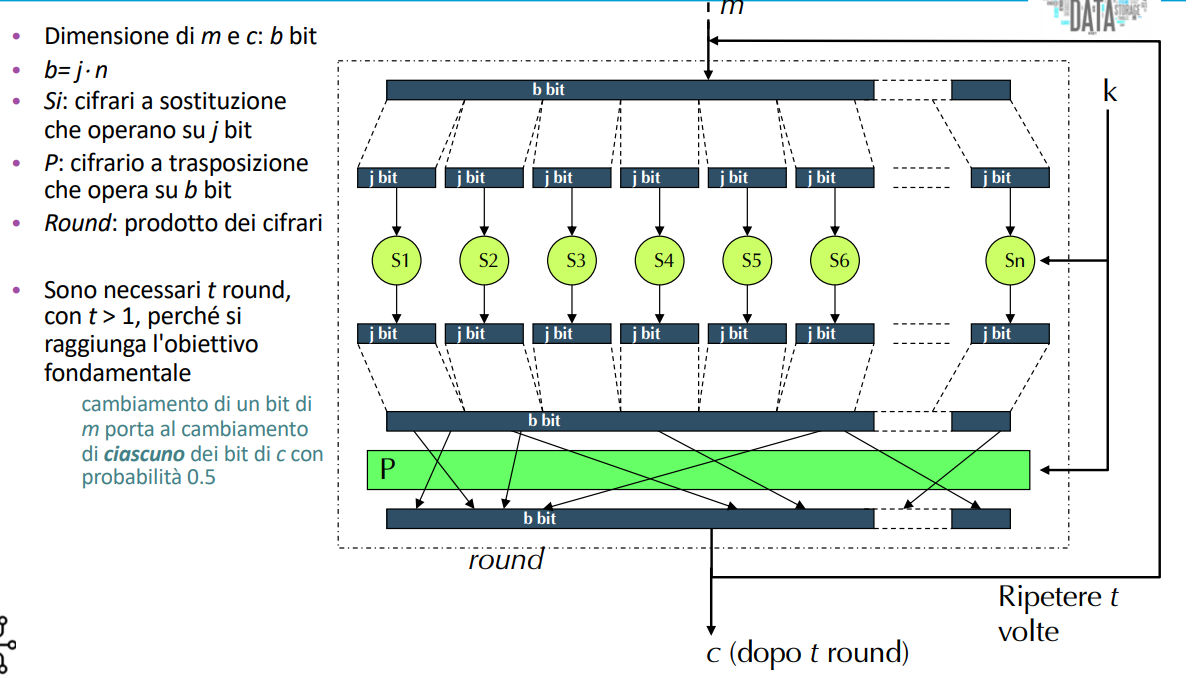
\includegraphics[width=\linewidth]{block-cypher-proto.png}
	\caption{Didascalia}
	\label{fig:etichetta}
\end{figure}

\subsection{Data Encryption Standard (DES)}
\begin{itemize}
	\item È un cifrario simmetrico a blocchi sviluppato da IBM su commissione della NSA e standardizzato nel 1977.
	\item Opera su blocchi di $b=64$ bit.
	\item Utilizza una chiave di $l=56$ bit (sebbene la chiave fornita sia di 64 bit, 8 bit sono di parità e vengono scartati).
	\item È basato su un \textbf{cifrario di tipo Feistel}, che divide il blocco in due metà (Sinistra L e Destra R) e applica 16 round.
	          
	      \begin{figure}[H]
	      	\centering
	      	\includegraphics[width=\linewidth]{des.png}
	      	\caption{DES schema ad alto livello}
	      	\label{fig:etichetta}
	      \end{figure}
	          
	          
	\item Lo stesso algoritmo (circuito) si usa per cifrare e decifrare, cambiando solo l'ordine di applicazione delle sottochiavi.
	          
	      \begin{figure}[H]
	      	\centering
	      	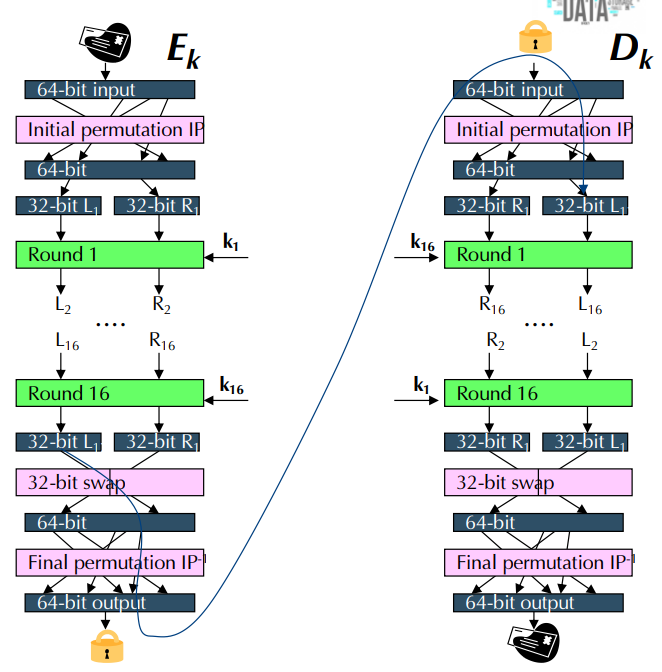
\includegraphics[width=\linewidth]{descomparison.png}
	      	\caption{DES: Encryption vs Decryption}
	      	\label{fig:etichetta}
	      \end{figure}
	          
	\item \textbf{Analisi:} La chiave a 56 bit ($2^{56}$ iterazioni) è oggi considerata insicura.
	      \begin{itemize}
	      	\item Già nel 1977 un attacco a forza bruta costava 20M\$ e richiedeva 12 ore.
	      	\item Nel 1993, 3.5 ore per 1M\$.
	      	\item Nel 2007 (COPACOBANA), meno di una settimana con 8K\$.
	      	\item Nel 2022, con 13 GPU (6000\$), si stima un tempo simile.
	      \end{itemize}
	\item \textbf{3DES (Triple DES):} Per sopperire alla chiave corta, oggi si usa il 3DES.
	      \begin{itemize}
	      	\item Applica DES tre volte con due chiavi (k1, k2): $c = E_{k1}(D_{k2}(E_{k1}(m)))$.
	      	\item La chiave effettiva diventa di $l=112$ bit ($2^{112}$ spazio delle chiavi).
	      	\item È retrocompatibile con DES (basta porre $k1=k2$).
	      \end{itemize}
	                
	      \begin{figure}[H]
	      	\centering
	      	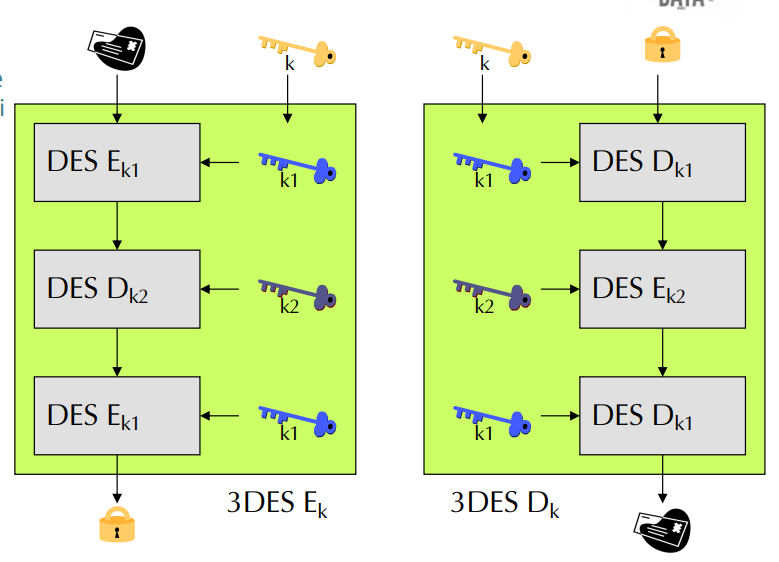
\includegraphics[width=\linewidth]{3DES.png}
	      	\caption{Il DES di oggi: 3DES}
	      	\label{fig:etichetta}
	      \end{figure}
	          
\end{itemize}

\subsection{Advanced Encryption Standard (AES)}
\begin{itemize}
	\item È il successore di DES, standardizzato nel 2001. Si basa sull'algoritmo \textbf{Rijndael}.
	\item Dimensione del blocco $b=128$ bit.
	\item Lunghezza chiave $l$ variabile: 128, 192 o 256 bit (AES-128, AES-192, AES-256).
	\item A differenza di DES, non è una rete di Feistel. Opera su "stati", ovvero matrici di $4 \times 4$ byte (per AES-128).
	\item Applica un numero di round che dipende dalla lunghezza della chiave (es. 9 round principali per AES-128).
	\item Ogni round è composto da 4 operazioni:
	      \begin{enumerate}
	      	\item \textbf{SubBytes:} Sostituzione non lineare di ogni byte usando una S-box.
	      	\item \textbf{ShiftRows:} Rotazione (shift) delle righe dello stato.
	      	\item \textbf{MixColumns:} Moltiplicazione di ogni colonna per una matrice (diffusione). (Assente nel round finale).
	      	\item \textbf{AddRoundKey:} XOR tra lo stato e la sottochiave del round.
	      \end{enumerate}
	                
	      \begin{figure}[H]
	      	\centering
	      	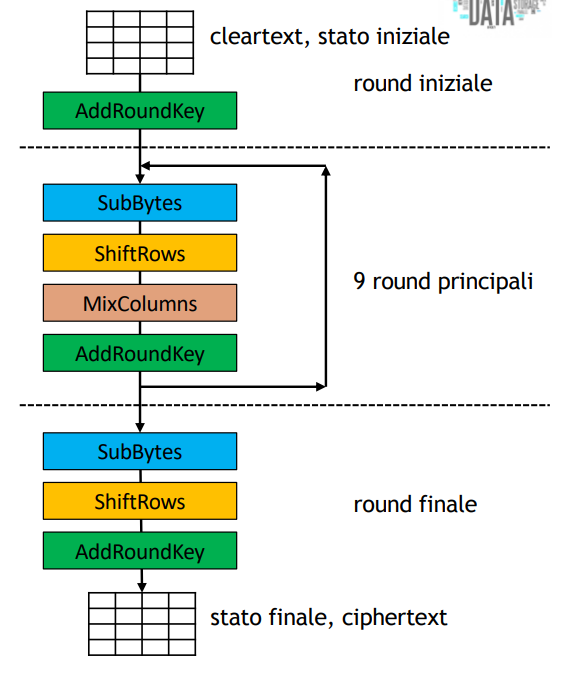
\includegraphics[width=\linewidth]{round-aes.png}
	      	\caption{AES: operazioni e round}
	      	\label{fig:etichetta}
	      \end{figure}
	          
	\item \textbf{Sicurezza:} Non si conoscono attacchi crittanalitici pratici più efficienti della forza bruta. La NSA lo approva per dati \emph{SECRET} (128 bit) e \emph{TOP-SECRET} (256 bit).
	\item È molto più veloce di DES/3DES, specialmente in SW.
\end{itemize}

\subsection{International Data Encryption Algorithm (IDEA)}
\begin{itemize}
	\item È un algoritmo a blocchi introdotto nel 1991, coperto da brevetto.
	\item Ha una dimensione di blocco $b=64$ bit.
	\item Utilizza una chiave di lunghezza $l=128$ bit, ritenuta sufficiente per proteggere da ricerche esaustive.
	\item È stato progettato per resistere a tecniche crittanalitiche avanzate, come la differential cryptanalysis.
	\item È progettato per essere efficiente sia in HW (grazie a strutture regolari) sia in SW (utilizzando operazioni orientate a multipli di ottetti, 16 bit, e funzioni base dei processori).
	\item Ad oggi, non sono stati pubblicati metodi pratici (oltre alla forza bruta) per violare IDEA.
	\item Viene utilizzato in diversi sistemi commerciali, tra cui PGP e S/MIME.
\end{itemize}

\subsection{Blowfish (BF)}
\begin{itemize}
	\item È un algoritmo a blocchi introdotto nel 1994 ed è royalty-free.
	\item Ha una dimensione di blocco $b=64$ bit.
	\item Si distingue per una lunghezza della chiave $l$ variabile, che può andare da 32 a 448 bit.
	\item È stato uno dei primi algoritmi a introdurre il concetto di sicurezza variabile, legata alla dimensione della chiave scelta.
	\item È stato progettato per essere estremamente efficiente in implementazioni software (SW) su processori general-purpose.
	\item Risulta, invece, molto meno efficace in implementazioni hardware (HW), a causa di un algoritmo di generazione delle sotto-chiavi complesso che richiede "molta" memoria.
	\item Sebbene abbia ricevuto meno attenzione (in termini di tempo) di IDEA, finora non sono stati trovati problemi seri.
\end{itemize}

\subsection{Stream Cipher}
\begin{itemize}
	\item \textbf{Block Cipher (BC):} Processano blocchi "larghi" ($b \ge 64$ bit) e sono \emph{stateless} (la stessa $E_k$ è usata per tutti i blocchi).
	\item \textbf{Stream Cipher (SC):} Processano blocchi "piccoli" ($1 \le b \le 8$ bit) e sono \emph{stateful} (la funzione di cifratura varia man mano).
	\item \textbf{One-Time-Pad:} È lo stream cipher perfetto, ma richiede una chiave (keystream) lunga quanto il messaggio e perfettamente casuale.
	\item Gli SC pratici generano un \emph{keystream pseudocasuale} $z_i$ a partire da una chiave corta $k$ e cifrano tramite XOR: $c_i = m_i \oplus z_i$.
	\item \textbf{Synchronous SC:} Il keystream $z_i$ è generato indipendentemente da $m_i$ e $c_i$. Sorgente e destinazione devono essere perfettamente sincronizzate. Se si perde un blocco, la decifrazione dei successivi è errata. (Es. RC4, Chacha-20, vedi pagine 32-33 slide symm).
	         
	      \subsubsection{Stream Cipher: Synchronous}
	      \begin{itemize}
	      	\item Gli stream cipher processano il plaintext in blocchi piccoli ($1 \le b \le 8$ bit) e sono \emph{stateful} (con memoria).
	      	\item L'idea è generare un \textbf{keystream pseudocasuale} ($z_i$) a partire da una chiave corta $K$ e cifrare tramite XOR.
	      	\item In un cifrario \emph{synchronous}, il keystream è generato indipendentemente dal plaintext e dal ciphertext.
	      	\item Il generatore di keystream mantiene uno \textbf{stato} interno $s_i$.
	      	\item \textbf{Cifratura:} $c_i = m_i \oplus z_i$.
	      	\item \textbf{Decifratura:} $m_i = c_i \oplus z_i$.
	      	\item Il keystream $z_i$ e lo stato successivo $s_{i+1}$ sono generati da due funzioni $g$ e $f$ che dipendono solo dallo stato corrente $s_i$ e dalla chiave $K$.
	      	\item \textbf{Proprietà:}
	      	      \begin{itemize}
	      	      	\item Mittente e destinatario devono essere perfettamente sincronizzati, partendo dallo stesso stato iniziale.
	      	      	\item La perdita o l'aggiunta di un singolo blocco durante la trasmissione rompe la sincronizzazione, rendendo errata la decifrazione di tutti i blocchi successivi.
	      	      	\item Non c'è propagazione dell'errore per i \emph{bit error}: un errore su un bit di $c_i$ corrompe solo il bit corrispondente in $m_i$, senza influenzare i blocchi successivi.
	      	      \end{itemize}
	      	\item \textbf{Sicurezza:} Non offre segretezza perfetta (alla Shannon) perché l'entropia della chiave è molto minore di quella del messaggio ($H(k) \ll H(m)$). La sicurezza si basa sulla impredicibilità del keystream pseudo-casuale.
	      \end{itemize}
	      
	      \begin{figure}[H]
	      	\centering
	      	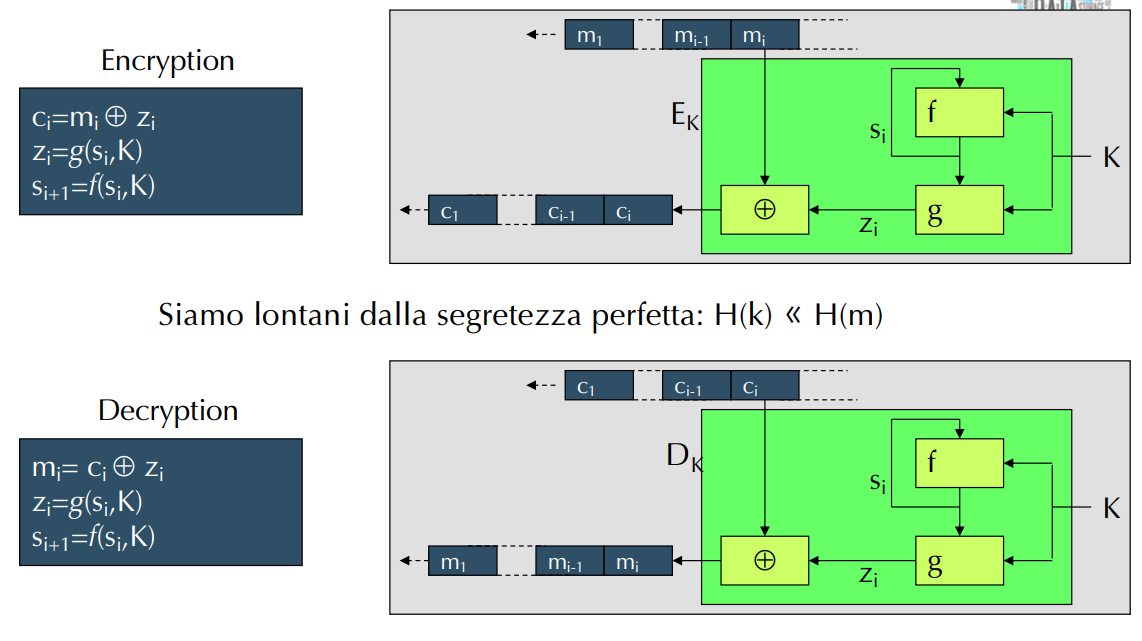
\includegraphics[width=\linewidth]{ssc.png}
	      	\caption{Schema Synchronous Stream Cipher}
	      	\label{fig:etichetta}
	      \end{figure}
	         
	\item \textbf{Self-synchronizing SC:} Il keystream $z_i$ dipende dalla chiave $k$ e dai $t$ blocchi di \emph{ciphertext} precedenti: $z_i = g(c_{i-1}, ..., c_{i-t}, K)$. Si auto-risincronizza dopo un errore: la perdita di un $c_i$ corrompe solo un numero limitato di $m_j$ successivi. 
	            
	      \subsubsection{Stream Cipher: Self-Synchronizing}
	      \begin{itemize}
	      	\item È un cifrario a flusso in cui il keystream $z_i$ dipende dalla chiave $K$ e da un numero finito $t$ di blocchi di \textbf{ciphertext} precedenti.
	      	\item \textbf{Cifratura:} $c_i = m_i \oplus z_i$, dove $z_i = g(c_{i-1}, \dots, c_{i-t}, K)$.
	      	\item \textbf{Decifratura:} $m_i = c_i \oplus z_i$, dove $z_i = g(c_{i-1}, \dots, c_{i-t}, K)$.
	      	\item \textbf{Initialization Vector (IV):} Per avviare il processo, è necessaria una serie di $t$ blocchi $v_i$ iniziali e non segreti, noti a mittente e destinatario.
	      	\item \textbf{Proprietà (Vantaggio):} È \textbf{auto-sincronizzante}. Se un blocco di $c_i$ viene perso o aggiunto, la decifrazione sarà errata solo per un numero limitato di blocchi successivi (dipendente da $t$). Dopodiché, il sistema si riallinea automaticamente.
	      	\item \textbf{Proprietà (Svantaggio):} \textbf{Propagazione dell'errore}. Un singolo errore (bit flip) su un blocco $c_i$ corrompe il plaintext $m_i$ e anche i $t$ blocchi successivi, portando alla corruzione di $t+1$ blocchi in chiaro.
	      \end{itemize}

	      \begin{figure}[H]
	      	\centering
	      	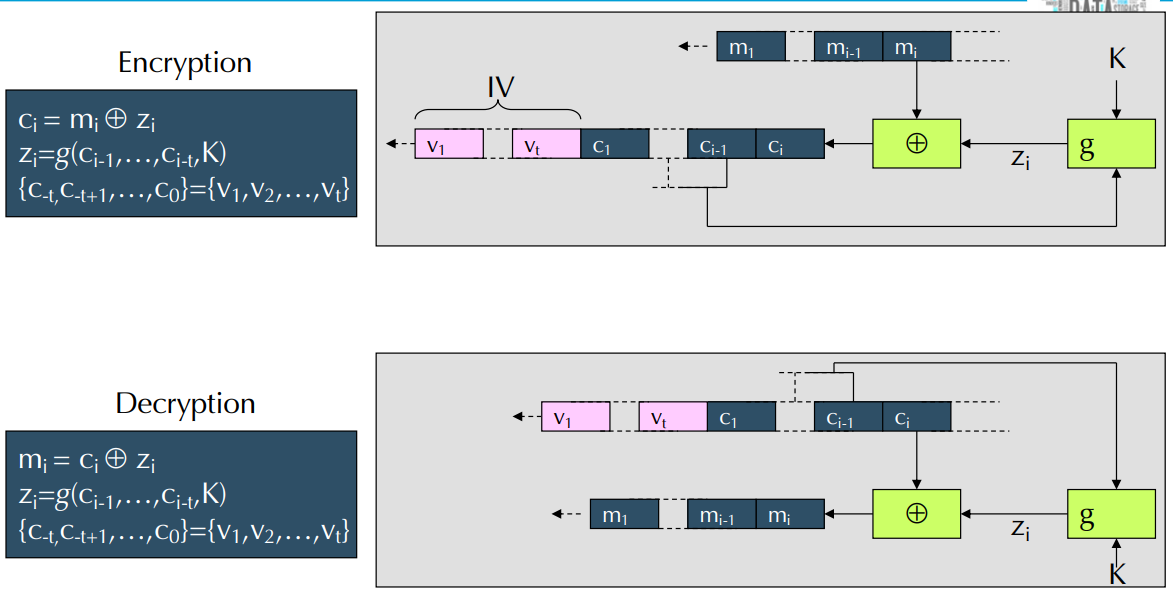
\includegraphics[width=\linewidth]{sssc.png}
	      	\caption{Schema Self-synchronizing Stram Cipher}
	      	\label{fig:etichetta}
	      \end{figure}
\end{itemize}

\subsection{Modi d'uso dei Block Cipher}
Sono meccanismi che permettono di usare i block cipher (stateless) per cifrare messaggi più lunghi della dimensione del blocco $b$, trasformandoli di fatto in stream cipher.

\begin{itemize}
	\item \textbf{Electronic Code Book (ECB):}
	      \begin{itemize}
	      	\item È il modo più semplice: ogni blocco $m_i$ è cifrato indipendentemente: $c_i = E_k(m_i)$.
	      	\item \textbf{Svantaggio:} Blocchi $m_i$ identici producono blocchi $c_i$ identici. Questo non nasconde le relazioni statistiche del plaintext ed è vulnerabile ad attacchi.
	      	\item \textbf{Non va mai usato}.
	      \end{itemize}
	                
	      \begin{figure}[H]
	      	\centering
	      	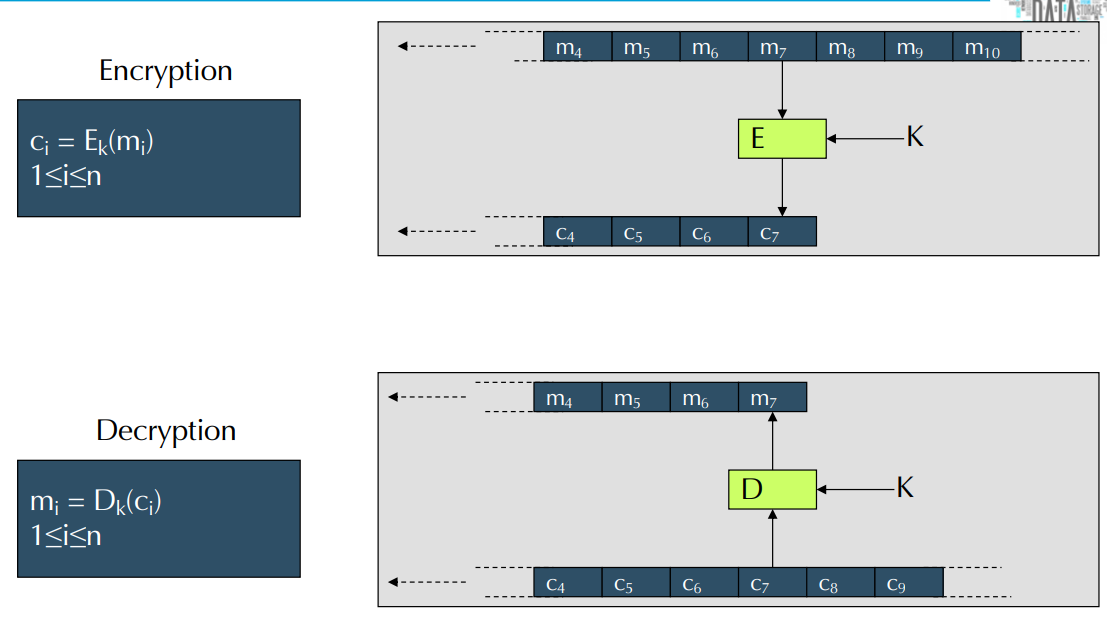
\includegraphics[width=\linewidth]{ECB.png}
	      	\caption{Electronic Code Book Mode}
	      	\label{fig:etichetta}
	      \end{figure}
	           
	\item \textbf{Cipher Block Chaining (CBC):}
            \begin{itemize}
              \item Introduce una dipendenza (chaining) tra i blocchi per nascondere le relazioni statistiche del plaintext.
              \item \textbf{Cifratura:} Come mostra l'immagine, il blocco di plaintext $m_i$ viene prima combinato in XOR con il blocco di \emph{ciphertext} precedente $c_{i-1}$. Il risultato di questo XOR viene poi cifrato con la chiave $K$.
              \item \textbf{Formula Cifratura:} $c_i = E_k(m_i \oplus c_{i-1})$.
              \item \textbf{Decifratura:} Il blocco $c_i$ viene prima decifrato con la chiave $K$. Il risultato ($D_k(c_i)$) viene poi combinato in XOR con il blocco di \emph{ciphertext} precedente $c_{i-1}$ per riottenere il plaintext $m_i$.
              \item \textbf{Formula Decifratura:} $m_i = D_k(c_i) \oplus c_{i-1}$.
              \item \textbf{Initialization Vector (IV):} Poiché $m_1$ non ha un $c_0$ precedente, si usa un blocco iniziale $IV$ (che può essere pubblico, ma deve essere casuale e imprevedibile) per avviare la catena: $c_0 = IV$.
              \item \textbf{Vantaggio:} Stessi blocchi $m_i$ producono $c_i$ diversi (a meno che anche i $c_{i-1}$ siano identici, evento improbabile). Resiste molto bene all'analisi della frequenza.
              \item \textbf{Svantaggio (Propagazione dell'Errore):} Un errore (es. un bit flip) in un singolo blocco $c_i$ corrompe la decifrazione di \textbf{due} blocchi:
                \begin{itemize}
                  \item $m_i$ viene completamente corrotto (perché $D_k(c_i)$ sarà incomprensibile).
                  \item $m_{i+1}$ viene corrotto solo parzialmente, negli stessi bit in cui $c_i$ era errato (perché $D_k(c_{i+1})$ è corretto, ma viene XORato con il $c_i$ errato).
                  \item L'errore si ferma qui; $m_{i+2}$ sarà decifrato correttamente (il sistema si auto-risincronizza).
                \end{itemize}
              \end{itemize} 
	                
	      \begin{figure}[H]
	      	\centering
	      	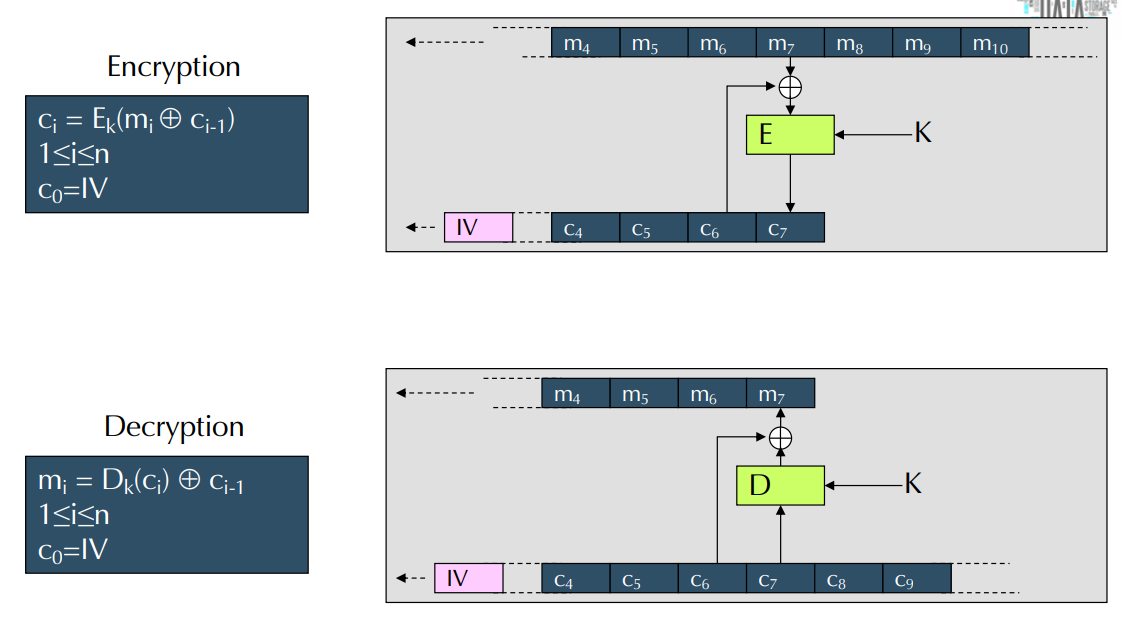
\includegraphics[width=\linewidth]{CBC.png}
	      	\caption{Cipher Block Chaining Mode}
	      	\label{fig:etichetta}
	      \end{figure}
	                
	\item \textbf{Counter Mode (CTR):}
	     \begin{itemize}
    \item Trasforma un block cipher in uno stream cipher di tipo \emph{synchronous}.
    \item \textbf{Generazione Keystream:} Genera un keystream $o_i$ (detto \emph{output block}) cifrando un \textbf{contatore} $p_i$.
    \item Il contatore $p_i$ è tipicamente generato combinando un \textbf{Initialization Vector (IV)} (o Nonce) con un numero che si incrementa per ogni blocco (es. $p_i = IV + i - 1$).
    \item \textbf{Cifratura:} Il plaintext $m_i$ è combinato in XOR con il keystream: $c_i = o_i \oplus m_i$.
    \item \textbf{Decifratura:} Avviene nello stesso modo. Si genera lo \emph{stesso identico} keystream $o_i$ (cifrando lo stesso contatore $p_i$) e lo si combina in XOR con il ciphertext $c_i$.
    \item \textbf{Formula Decifratura:} $m_i = o_i \oplus c_i$.
    \item \textbf{Nota Importante:} Come mostra il diagramma, sia la cifratura che la decifratura usano la funzione di \textbf{cifratura} $E_k$. La funzione di decifratura $D_k$ non è necessaria.
    \item \textbf{Vantaggio (Random Access):} È possibile calcolare il keystream $o_j$ e decifrare $m_j$ (avendo $c_j$) in modo indipendente, senza dover calcolare i $j-1$ blocchi precedenti. Questo permette l'accesso e la decifratura parallela (molto veloce) ed è ideale per la crittografia di dati ad accesso casuale (file, dischi, ecc.).
\end{itemize}
	                
	      \begin{figure}[H]
	      	\centering
	      	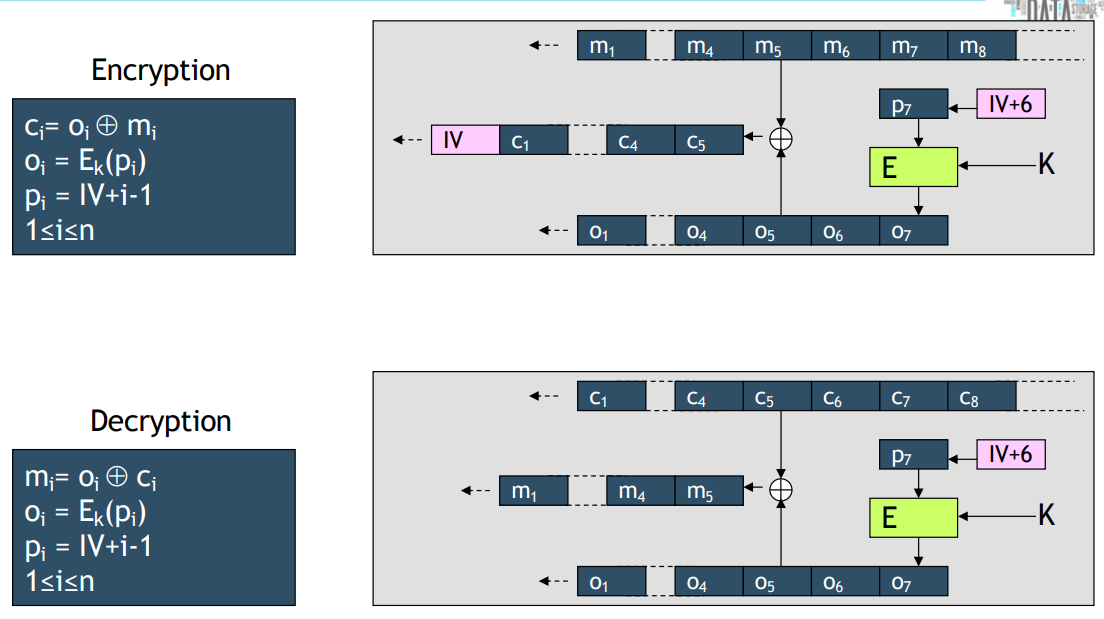
\includegraphics[width=\linewidth]{CTR.png}
	      	\caption{Schema modo Counter Mode}
	      	\label{fig:etichetta}
	      \end{figure}
\end{itemize}

\label{sec:funzioni-hash}

\subsection{Definizioni e Tipologie}
\begin{itemize}
	\item Una \textbf{funzione di hash} (o \emph{message digest function}) $h$ è una funzione che mappa una stringa binaria $m$ di lunghezza arbitraria in una stringa binaria $d$ (l'hash) di lunghezza $n$ fissa.
	\item L'hash $d=h(m)$ è una "impronta digitale" (fingerprint) o rappresentazione compatta di $m$.
	\item \textbf{MDC (Modification Detection Code):}
	      \begin{itemize}
	      	\item È una funzione di hash \emph{senza chiave}: $d = h(m)$.
	      	\item \textbf{Obiettivo:} Garantire l'integrità di $m$. Se l'hash $d$ (ottenuto separatamente, es. da un sito web) è integro, si può verificare che $m$ non sia stato modificato.
	      \end{itemize}
	\item \textbf{MAC (Message Authentication Code):}
	      \begin{itemize}
	      	\item È una funzione di hash \emph{con chiave} (segreta): $d = h_k(m)$.
	      	\item \textbf{Obiettivo:} Garantire sia l'integrità (nessuno ha modificato $m$) sia l'autenticazione (solo chi conosce $k$ può aver generato $d$).
	      \end{itemize}
\end{itemize}

\begin{figure}[H]
	\centering
	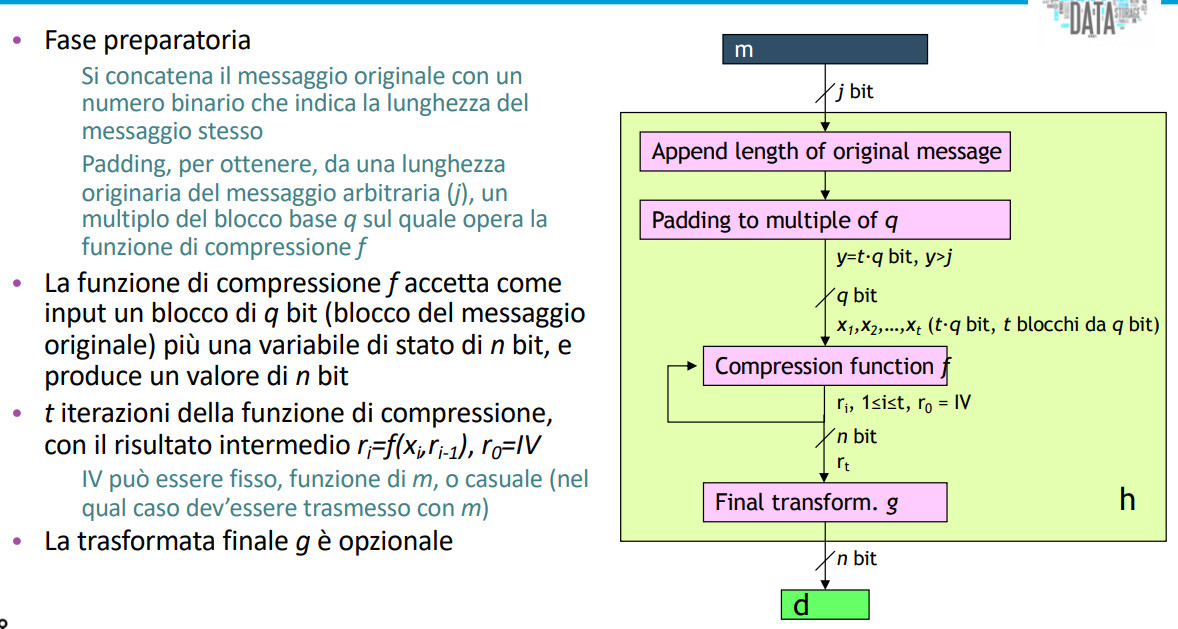
\includegraphics[width=\linewidth]{MDC.png}
	\caption{Modello MDC (funzione di hash iterativa)}
	\label{fig:etichetta}
\end{figure}

\subsection{Proprietà di Sicurezza (MDC)}
Una funzione di hash crittografica (MDC) deve avere le seguenti proprietà:
\begin{itemize}
	\item \textbf{Efficienza:} Deve essere semplice calcolare $d=h(m)$.
	\item \textbf{Preimage Resistance (Non invertibilità):} Dato $d$, deve essere computazionalmente difficile risalire a $m$ tale che $h(m)=d$.
	\item \textbf{2nd Preimage Resistance (Weak Collision Resistance):} Dato $x$, deve essere computazionalmente difficile trovare un $y \neq x$ tale che $h(y) = h(x)$.
	\item \textbf{Strong Collision Resistance:} Deve essere computazionalmente difficile trovare \emph{qualsiasi} coppia di messaggi distinti $(x, y)$ tali che $h(x) = h(y)$.
	\item \textbf{Paradosso del Compleanno (Birthday Problem):} A causa del paradosso del compleanno, la probabilità di trovare una collisione (strong collision) è 0.5 dopo aver calcolato solo $O(2^{n/2})$ hash, dove $n$ è la dimensione dell'hash.
	\item Un MDC è sicuro se trovare collisioni richiede un lavoro $O(2^{n/2})$ e la preimage resistance è garantita.
\end{itemize}

\subsection{Algoritmi Notevoli (MDC e MAC)}
\begin{itemize}
	\item \textbf{MD5 (Message Digest 5):}
	      \begin{itemize}
	      	\item Introdotto nel 1991, produce un hash $n=128$ bit.
	      	\item È molto veloce.
	      	\item \textbf{È considerato insicuro:} Dal 1996 è stata dimostrata una crescente insicurezza. Nel 2005 è stato dimostrato che bastano 8 ore per trovare due messaggi che collidono (violazione della \emph{strong collision resistance}).
	      \end{itemize}
	\item \textbf{SHA-1 (Secure Hashing Algorithm 1):}
	      \begin{itemize}
	      	\item Introdotto nel 1993, produce un hash $n=160$ bit.
	      	\item Produce un digest più lungo di MD5 (160 vs 128) per resistere meglio al birthday attack.
	      	\item \textbf{È considerato insicuro:} Nel 2005 è stata mostrata la sua insicurezza teorica (trovare collisioni richiede $O(2^{69})$ operazioni invece del $O(2^{80})$ ottimale).
	      \end{itemize}
	\item \textbf{HMAC (Hash-based MAC):}
	      \begin{itemize}
	      	\item È un metodo standard per costruire un MAC sicuro a partire da un qualsiasi MDC (es. HMAC-SHA1).
	      	\item La formula è: $MAC_k(m) = MDC((k \oplus c_1) | MDC((k \oplus c_2) | m))$ (dove $k$ è paddato e $c_1, c_2$ sono costanti).
	      	\item \textbf{Vantaggio:} È un meccanismo la cui sicurezza è dimostrata. L'applicazione di HMAC "risolve" i problemi di bassa collision-resistance degli MDC sottostanti (come MD5). Per questo, \textbf{usate HMAC}.
	      \end{itemize}
\end{itemize}

\end{document}
